\documentclass[a4paper]{article}
\usepackage{cmap}
\usepackage{mathtext}
\usepackage{amssymb}
\usepackage{amsmath}
\usepackage{wrapfig}
\usepackage[russian]{babel}
\usepackage{indentfirst}
\usepackage[pdftex]{graphicx}
\usepackage{multirow}
\usepackage{mathrsfs}
\usepackage{biblatex}
\usepackage{siunitx}
\usepackage[left=2cm,right=2cm,top=2cm,bottom=2cm]{geometry}
\usepackage{fancyhdr}
\bibliography{bib}
\pagestyle{fancy}
\newcommand{\const}{\mathrm{const}}
\newcommand{\rref}[1]{(\ref{#1})}
\newcommand{\isotope}[2]{$ ^{#2}\mathrm{#1} $}
\newenvironment{comment}{}{}
\newcommand{\picref}[1]{рис. \ref{#1}}
\newcommand{\mbf}{\mathbf}
\newcommand{\gmm}{$\gamma $}
\newcommand{\Equip}[3]{
	
	\item{\bf #1:} $\Delta = \pm #2\; #3$}
\newcommand{\equip}[1]{
	
	\item{\bf #1}}
\newcommand{\labname}{Изучение спектров атомов водорода и молекул йода} 	% название пиши здесь
\newcommand{\labnum}{5.2.2/5.2.3}		% номер вводи здесь
\renewcommand{\epsilon}{\varepsilon}
\renewcommand{\phi}{\varphi}
\newcommand{\angstrom}{\text{\AA}}
\fancyfoot{}
\fancyhead[RE, RO]{\thepage}
\fancyhead[LE, LO]{Лабораторная работа \labnum \space \labname}
\title{Лабораторная работа \labnum \space \labname}
\author{Иван Сладков}
\begin{document}
	\maketitle
	\thispagestyle{empty}
	\section{Аннотация}
	В данной работе проводится исследование спектральных закономерностей в оптических спектрах водорода и йода. По результатам измерений вычисляются постоянная Ридберга для водорода и потенциал ионизации. Кроме того, вычисляется энергия колебательного кванта молекулы йода и энергия ее диссоциации в основном и возбужденном состояниях.
	
	\section{Теоретические сведения}
	
	\paragraph{Спектр атомов водорода.}
	
	Объяснение структуры спектра излучения атомов требует решения задачи о движении электрона в эффективном поле атома.	Для атома водорода и водородоподобных (одноэлектронных) атомов 	определение энергетических уровней значительно упрощается, так как	квантово-механическая задача об относительном движении электрона (заряд $ -e $, масса $ m_e $) и ядра (заряд $ Z_e $, масса $ M $) сводится к задаче о движении частицы с эффективной массой $ \mu = m_e M /(m_e+M) $ в кулоновском поле $ - Z \epsilon^2 / n $. Длины волн спектральных линий водородоподобного атома описываются формулой
	\begin{equation}\label{key}
		\dfrac{1}{\lambda_{m n}} = R Z^2 (\dfrac{1}{n^2}-\dfrac{1}{m^2}),
	\end{equation}
	где $ m, \;n \in \mathbb{Z} $, а $ R $ -- постоянная Ридберга.
	Эта формула позволяет по энергиям перехода судить о расположении энергетических уровней атома водорода. На рис. \ref{fig:screenshot1} изображены энергетические уровни и соответствующие им переходы, определяющие спектр.
	\begin{wrapfigure}{}{0.5\textwidth}
		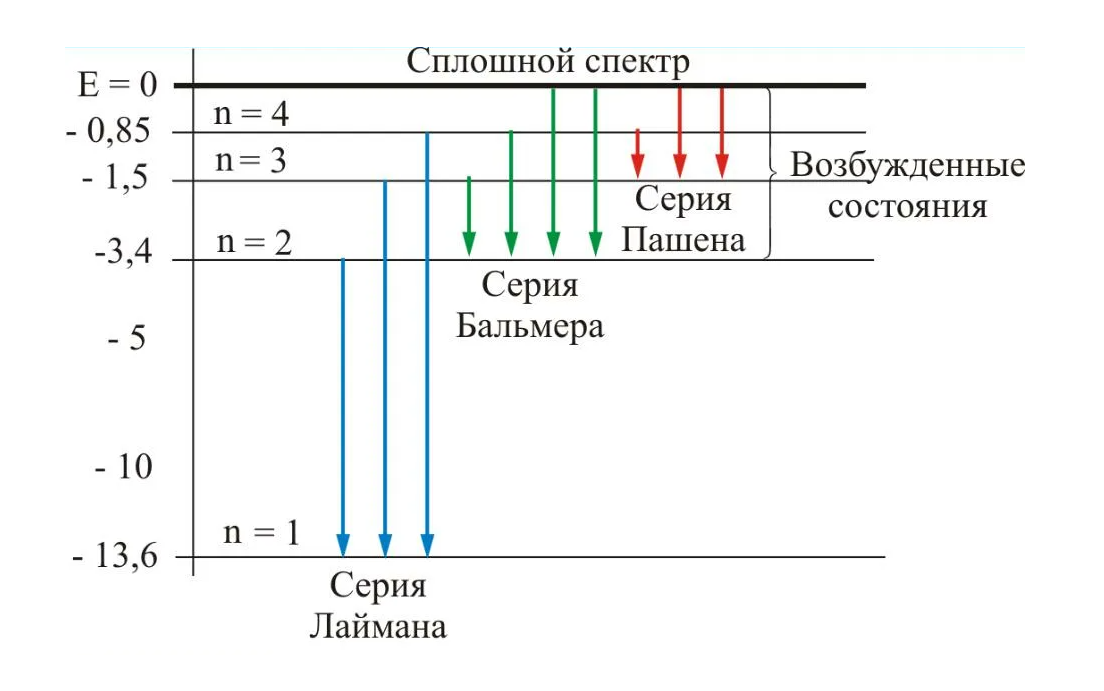
\includegraphics[width=1.0\linewidth]{Screenshot_1}
		\caption{Энергетические уровни атома водорода}
		\label{fig:screenshot1}
	\end{wrapfigure}
	В данной работе изучается серия Бальмера, линии которой лежат в видимой области. Для серии Бальмера $ n = 2 $. Величина $ m $ для первых четырех линий этой серии принимает значение 3, 4, 5, 6. Эти линии	обозначаются символами $ H_\alpha,\;H_\beta,\;H_\gamma,\;H_\delta $.
	
	Оценим энергии основного и возбужденного состояний водородоподобного атома. Чтобы найти основное состояние квантовой системы, надо минимизировать, с учетом соотношения неопределенностей, полную энергию. Потенциальная энергия электрона равна кулоновской энергии электрона в поле ядра с зарядом $ Z e $. Так как электрон локализован в области размером $ r $, то его импульс $ p \simeq \hbar / r $, и полная энергия определяется выражением
	\begin{equation}\label{eq:energy}
		E = \dfrac{-Z e^2}{r}+\dfrac{\hbar^2}{2 m_e r^2}.
	\end{equation}
	Приняв за нуль производную этого выражения, получим
	\begin{equation*}\label{key}
		r_Б = \dfrac{\hbar^2}{Z m_e e^2}.
	\end{equation*}
	Это значение радиуса первой орбиты для электрона в поле ядра с зарядом $ Z $ -- боровского радиуса. Подставляя в \eqref{eq:energy} это значение, получим
	\begin{equation*}\label{key}
		E = -R Z^2,
	\end{equation*}
	\begin{equation}\label{key}
		R = \dfrac{m_e e^4}{2 \hbar^2}.
	\end{equation}
	Для возбуждённых состояний значения энергий можно найти аналогично, приняв во внимание, что $ p \simeq n \hbar / r $ из условия, что на длине орбиты укладывается целое число волн де Бройля. Отсюда энергия $ n $-го уровня равна 
	\begin{equation*}\label{key}
		E = \dfrac{-R Z^2}{n^2}.
	\end{equation*}
	
	\paragraph{Спектр молекул йода.}
	
	\begin{wrapfigure}{}{0.5\textwidth}
		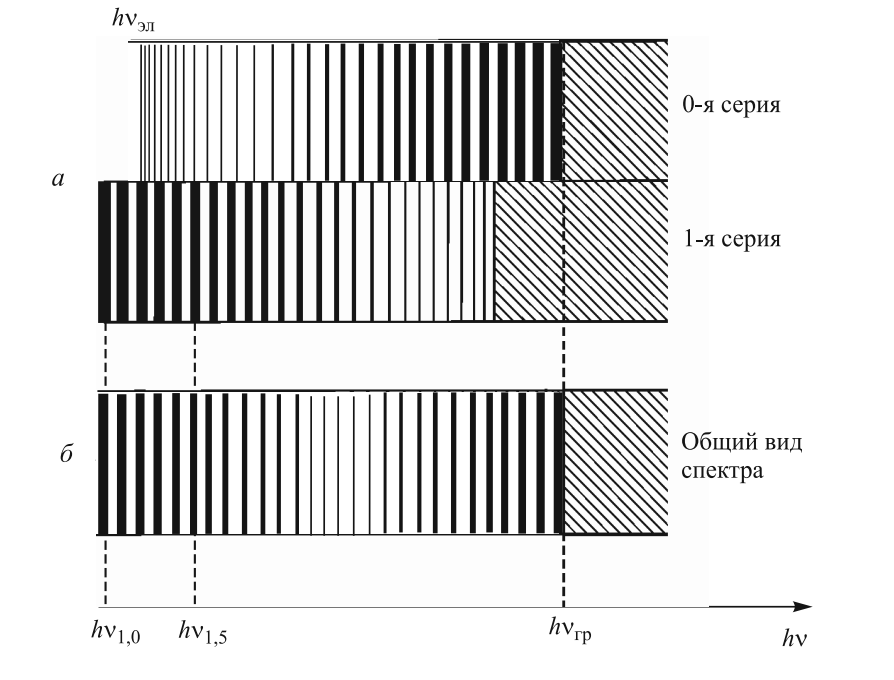
\includegraphics[width=1.0\linewidth]{Screenshot_3}
		\caption{Спектральная картина йода}
		\label{fig:screenshot3}
	\end{wrapfigure} 
	Массы ядер атомов велики по сравнению с массой электрона. Благодаря такой разнице в массах, скорости движения ядер в молекуле малы по сравнению со скоростями электронов. Это даёт возможность	рассматривать электронное движение при неподвижных ядрах, расположенных на определенных расстояниях друг от друга. Определяя уровни энергии такой системы, мы найдем электронные термы молекул. Любой атом в молекуле находится в электрическом поле остальных ее атомов. Оно вызывает расщепление электронных уровней атомов в молекуле. Следует отметить, что при соединении атомов в молекулу заполненные оболочки атомов мало меняются. Существенно может измениться распределение электронной плотности в не до конца заполненных оболочках.
	
	
	Спектр молекулярного йода представлен на рис. \ref{fig:screenshot3}.
	Для расчёта спектра поглощения йода необходимо учесть энергии колебательного и вращательного движения молекул. Видимый спектр состоит из 0-й и 1-й серий Деландра. 2-я серия в 10 раз менее интенсивная, чем 0-я, и поэтому ей пренебрегаем. 
	
	Энергетическое	положение линий поглощения описывается выражением
	\begin{equation}\label{eq:йод}
		h \nu_{0 n_2} = (E_2 - E_1 )+ h \nu_2 \left(n_2+\dfrac{1}{2}\right) - \dfrac{1}{2}h \nu_1.
	\end{equation}
%	\begin{wrapfigure}{}{0.3\textwidth}
%		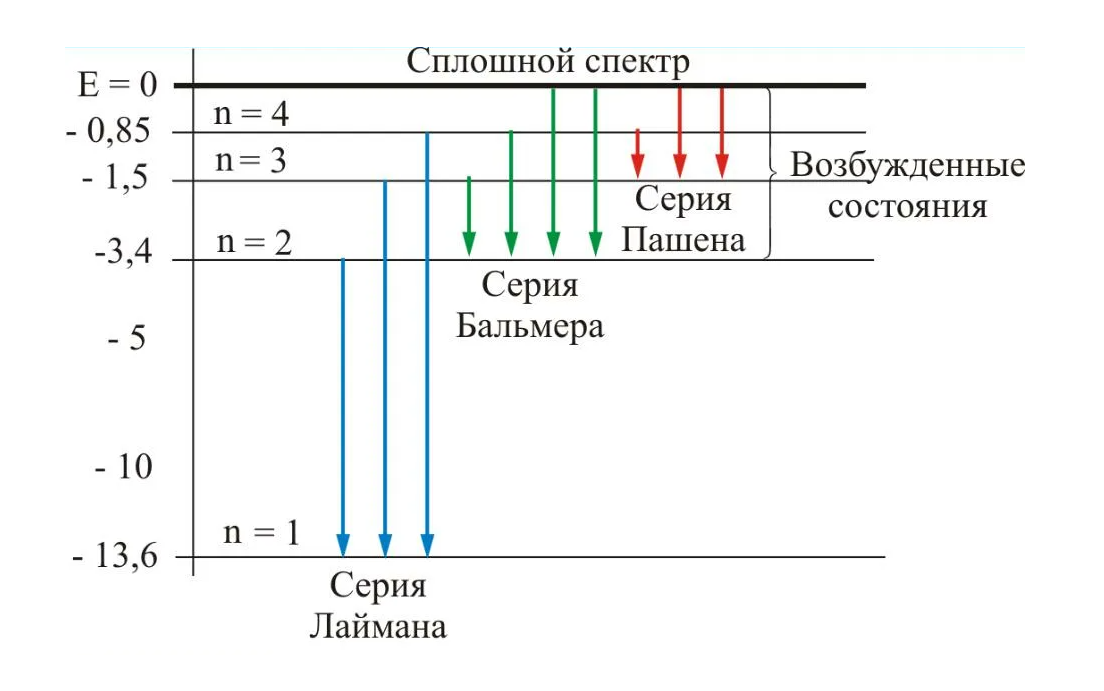
\includegraphics[width=1.0\linewidth]{Screenshot_1}
%		\caption{Энергетические уровни атома водорода}
%		\label{fig:screenshot1}
%	\end{wrapfigure}


		
	\section{Оборудование и инструментальные погрешности}
	
	\begin{figure}[hb]
		\centering
		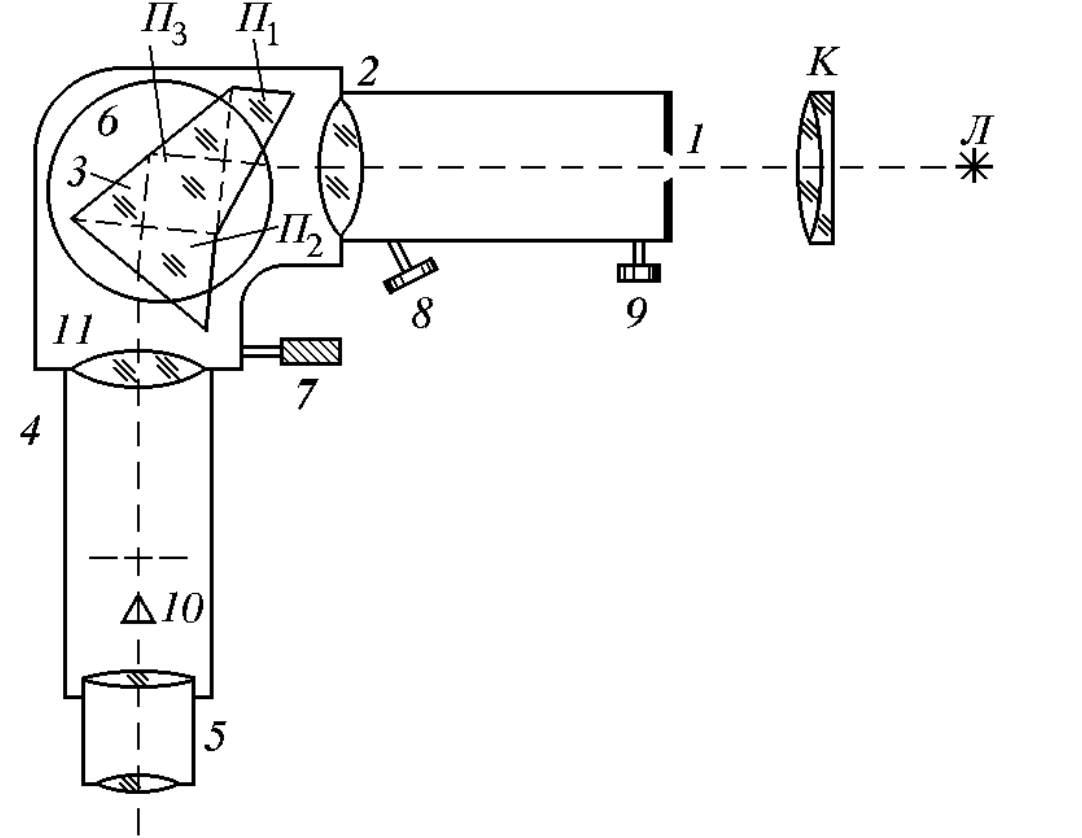
\includegraphics[width=0.6\textwidth]{Screenshot_2}
		\caption{Схема экспериментальной установки}
		\label{fig:screenshot2}
	\end{figure}
	
	
	Схема экспериментальной установки отображена на рис. \ref{fig:screenshot2}. Используется монохроматор, построенный на системе призм.
		
	В работе используются:
	\begin{itemize}
		\Equip{Монохроматор УМ-2}{2}{^\circ}
		\equip{Коллиматор}
		\equip{Водородная лампа}
		\equip{Кювета с кристаллами йода}
		\equip{Лампа накаливания на штативе}
		\equip{Неоновая и ртутная лампы}
	\end{itemize}
	
	\section{Результаты измерений и обработка данных}
	
	\subsection{Калибровка}
	
	Построим калибровочный график по спектрам неона и ртути на рис. \ref{fig:graph1}. Зависимость нелинейная, но аппроксимируется экспоненциальной функцией:
	\begin{equation}\label{eq:calibre}
		\lambda\left[\angstrom\right] = 234*\exp \left(\dfrac{\phi}{1105}\right)+3640.
	\end{equation}
	Для компактности формулу погрешностей здесь не приводим.
	\begin{figure}[hb]
		\centering
		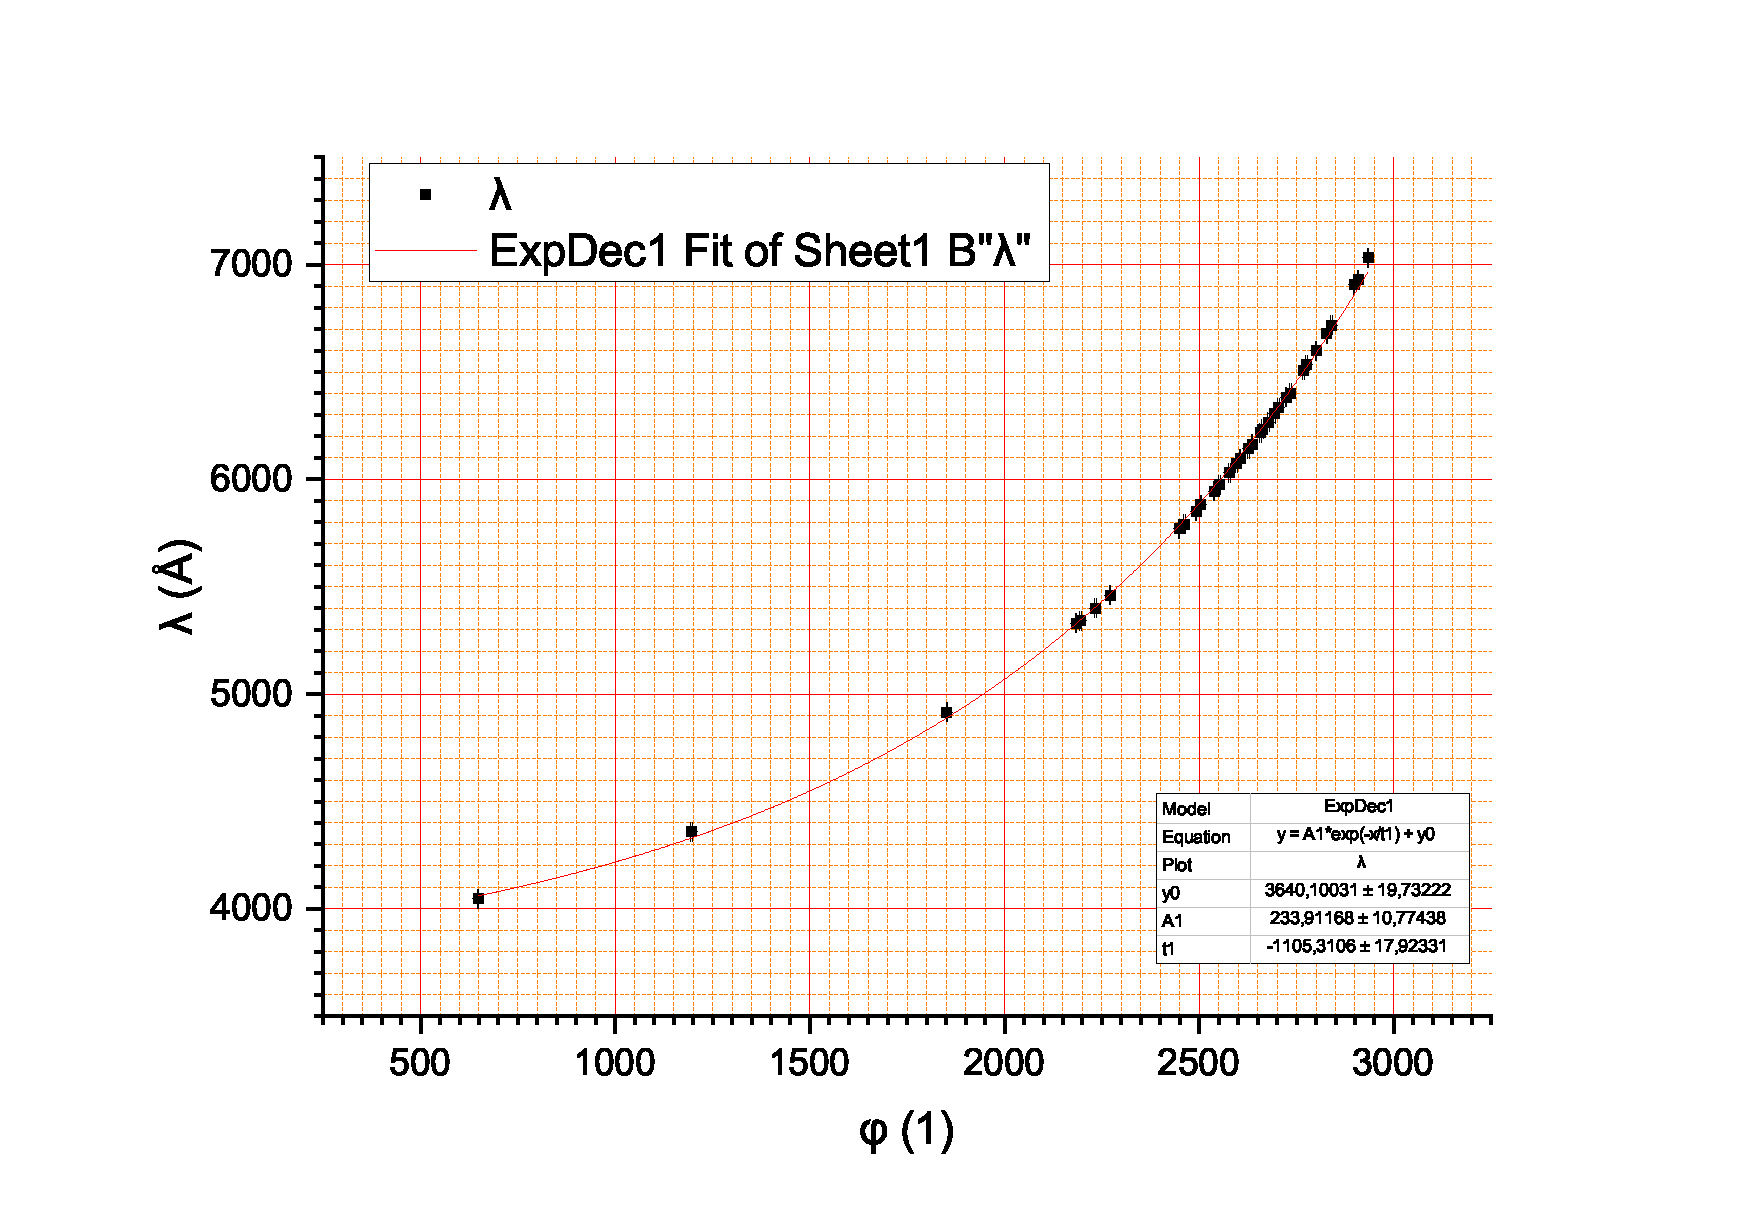
\includegraphics[width=0.8\linewidth]{Graph1}
		\caption{Калибровочный график по линиям водорода и йода}
		\label{fig:graph1}
	\end{figure}
	
	\subsection{Исследование спектров}
	
	Определим длины волн $H_\alpha,\;H_\beta,\;H_\gamma,\;H_\delta $ при помощи полученной калибровочной формулы \eqref{eq:calibre}. Результаты в табл. \ref{tab:H}:
	\begin{table}[h]
		\centering
		\begin{tabular}{|l|l|l|}
			\hline
			& $\phi, \;^\circ$ & $\lambda, \angstrom$ \\ \hline
			$ H_\alpha$ & $2792\pm 2$      & $6570\pm 190$        \\ \hline
			$H_\beta$   & $1804\pm 2$      & $4840\pm 70$         \\ \hline
			$H_\gamma$  & $1167\pm 2$      & $4310\pm 40$         \\ \hline
			$H_\delta$  & $763\pm 2$       & $4110\pm 30$         \\ \hline
		\end{tabular}
		\caption{Спектральные линии водорода}
		\label{tab:H}
	\end{table}
	В пределах погрешности полученные значения совпадают с табличными для серии Бальмера. Определим постоянную Ридберга. Построим график зависимости $ \lambda^{-1} $ от выражения вида $ 1/2 - 1/m^2 $ на рис.
	\begin{figure}
		\centering
		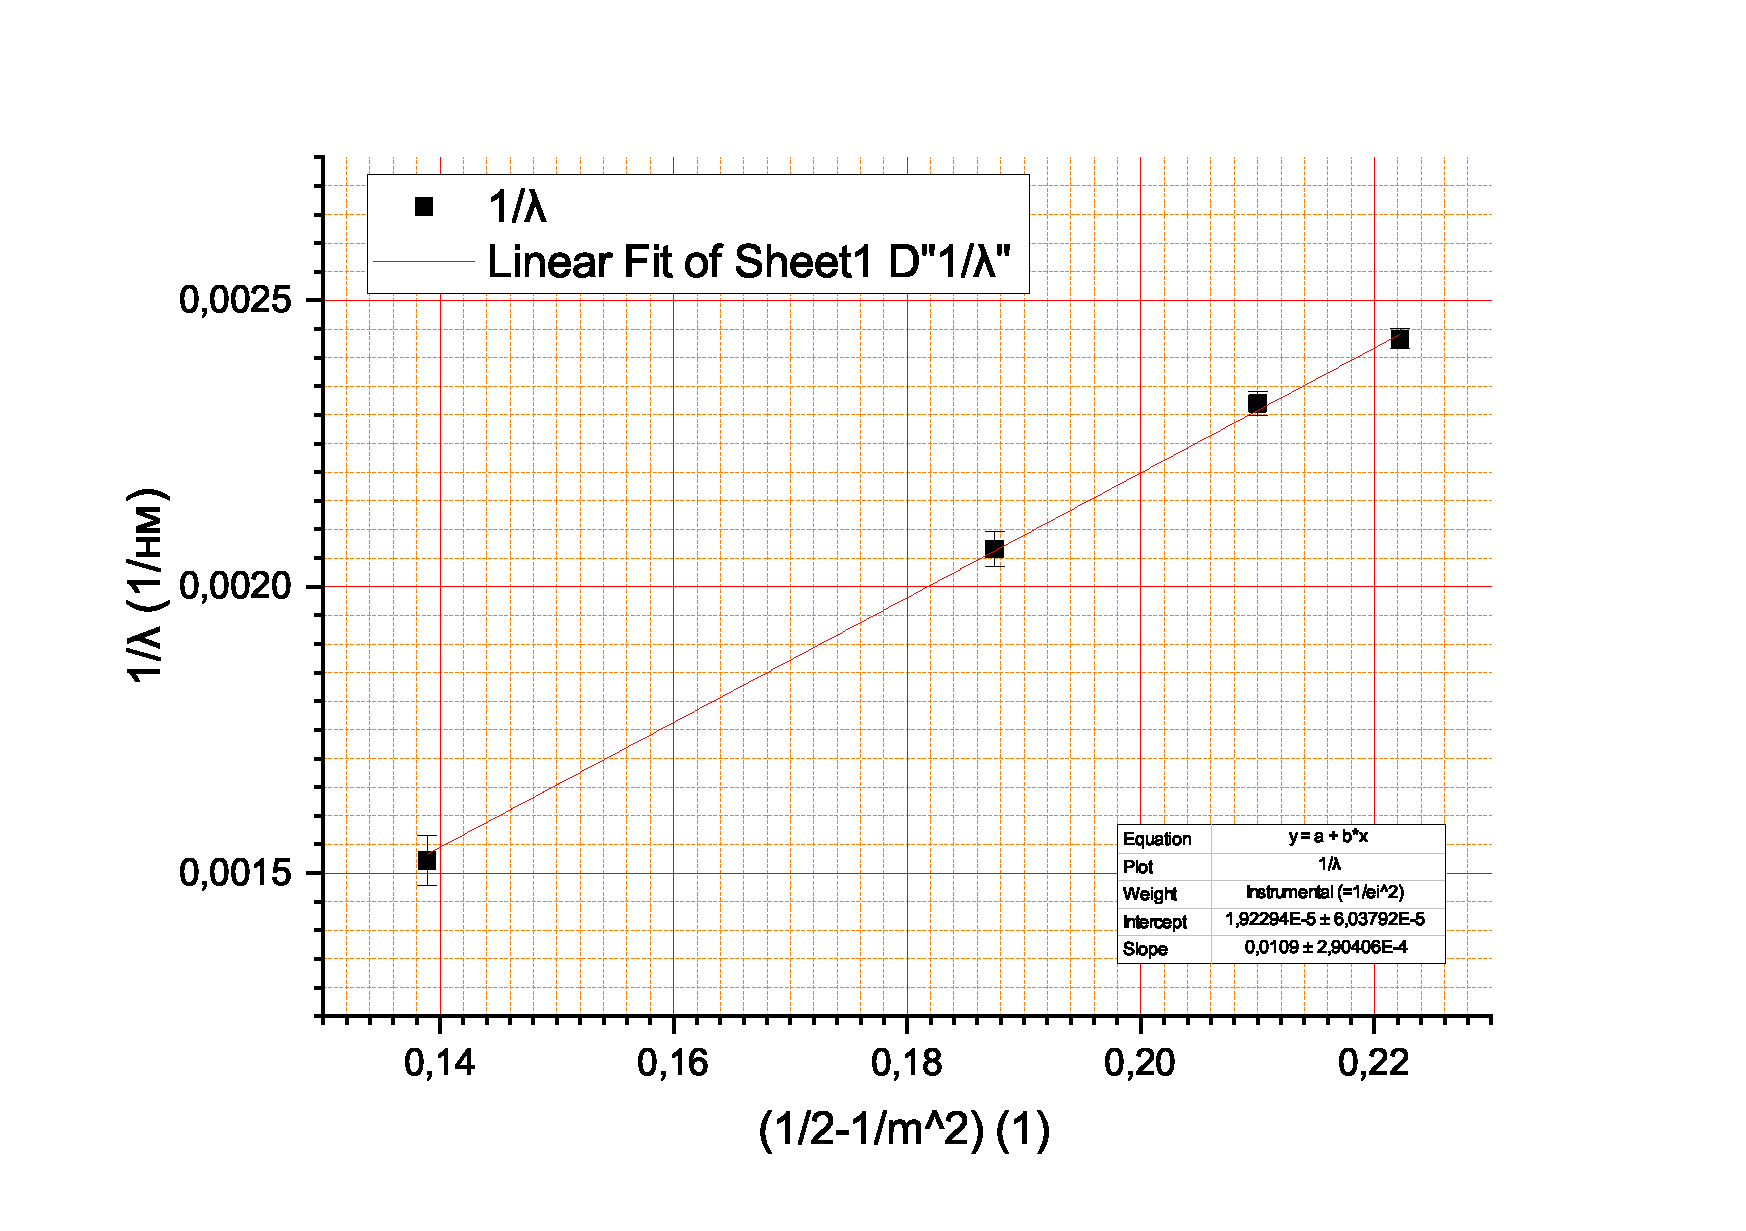
\includegraphics[width=0.7\linewidth]{Graph3}
		\caption{Зависимость $ \lambda^{-1} $ от $ 1/2 - 1/m^2 $}
		\label{fig:graph3}
	\end{figure}
	Из графика видно, что $ k = (109\pm 3)\cdot 10^{-4} $. Тогда
	\[R = k*10^9 = (1.09\pm 0.03)\cdot 10^7\; см^{-1}.\] Это значение совпадает с табличным в пределах погрешности.
	
	Найдём длины волн для йода:
	\[\nu_{1, 0} = 6096\pm 15\; \angstrom\]
	\[\nu_{1, 5} = 5880\pm 10 \;\angstrom\]
	\[\nu_{гр} = 5020\pm 10 \;\angstrom\]
	Вычислим в электрон-вольтах энергию колебательного кванта возбуждённого состояния молекулы йода:
	\[h\nu_2 = 15 \;мэВ.\]
	
	Найдём параметры диссоциации молекул йода:
	\[h\nu_{эл} = h\nu_{1, 0}+\dfrac{3}{2}h\nu_1 - \dfrac{1}{2}h\nu_2 = 2.13\pm 0.03\; эВ.\]
	Эта величина получена из формулы \eqref{eq:йод}. Тогда для энергии диссоциации частиц в основном и возбуждённом состояниях:
	\[D_1 = h\nu_{гр} - E_A = 1.48\pm 0.02\; эВ,\]
	\[D_2 = h\nu_{гр} - h\nu_{эл} = 0.28\pm 0.02\; эВ.\]
	Здесь $ E_A = 0,94\; эВ$ -- энергия возбуждения атома.
	
	\subsection{Оценка погрешностей}
		
	В данной работе оценка погрешностей при калибровке проведена по следующей формуле:
	\begin{equation}\label{eq:погр}
		\Delta \lambda = \sqrt{\frac{e^{-\frac{2 \phi}{t}} \left(a^2 \left(t^2 \sigma _\phi^2+\phi^2 \sigma _t^2\right)+t^4 \sigma _a^2\right)}{t^4}+\sigma _{\text{y0}}^2},
	\end{equation}	
	которая получена из общей формулы расчета погрешностей при помощи пакета \emph{Wolfram Mathematica}. Все погрешности были рассчитаны по общей формуле:
	\begin{equation}\label{eq:погрешности}
		\Delta_{u(x, y, z, \ldots)}^2 = f'^2_{x} \Delta_x^2 + f'^2_y \Delta_y^2 + f'^2_z \Delta_z^2 + \ldots,
	\end{equation}
	
	\section{Вывод}
	
	По результатам работы, получены характеристики спектров йода и водорода, по которым расчитаны свойства их молекул и атомов соответственно. Получены: постоянная Ридберга для водорода, а также энергия колебательного кванта молекулы йода, а также энергия диссоциации молекулы йода в основном и возбуждённом состояниях.
	
	\appendix
	\section{Необработанные результаты опытов}
	
	Данные, использованные для построения калибровочных графиков, представлены в табл. \ref{tab:raw}.
	
	\begin{table}[h]
		\centering
	\begin{tabular}{|l|l|l|}
		\hline
		$\phi, \;^\circ$ & $\lambda, \;\angstrom$ & $\Delta \phi, \;^\circ$ \\ \hline
		2934             & 7032                   & \multirow{33}{*}{2}     \\ \cline{1-2}
		2908             & 6929                   &                         \\ \cline{1-2}
		2840             & 6717                   &                         \\ \cline{1-2}
		2828             & 6678                   &                         \\ \cline{1-2}
		2800             & 6599                   &                         \\ \cline{1-2}
		2776             & 6533                   &                         \\ \cline{1-2}
		2768             & 6507                   &                         \\ \cline{1-2}
		2734             & 6402                   &                         \\ \cline{1-2}
		2723             & 6383                   &                         \\ \cline{1-2}
		2704             & 6334                   &                         \\ \cline{1-2}
		2693             & 6305                   &                         \\ \cline{1-2}
		2678             & 6267                   &                         \\ \cline{1-2}
		2658             & 6217                   &                         \\ \cline{1-2}
		2636             & 6164                   &                         \\ \cline{1-2}
		2626             & 6143                   &                         \\ \cline{1-2}
		2605             & 6096                   &                         \\ \cline{1-2}
		2596             & 6074                   &                         \\ \cline{1-2}
		2577             & 6030                   &                         \\ \cline{1-2}
		2552             & 5976                   &                         \\ \cline{1-2}
		2538             & 5945                   &                         \\ \cline{1-2}
		2504             & 5882                   &                         \\ \cline{1-2}
		2492             & 5852                   &                         \\ \cline{1-2}
		2233             & 5401                   &                         \\ \cline{1-2}
		2195             & 5341                   &                         \\ \cline{1-2}
		2184             & 5331                   &                         \\ \cline{1-2}
		2898             & 6907                   &                         \\ \cline{1-2}
		2662             & 6234                   &                         \\ \cline{1-2}
		2462             & 5791                   &                         \\ \cline{1-2}
		2448             & 5770                   &                         \\ \cline{1-2}
		2271             & 5461                   &                         \\ \cline{1-2}
		1852             & 4916                   &                         \\ \cline{1-2}
		1196             & 4358                   &                         \\ \cline{1-2}
		648              & 4047                   &                         \\ \hline
	\end{tabular}
		\caption{Необработанные данные калибровки}
		\label{tab:raw}
	\end{table}
	
	\begin{thebibliography}{3}
		\bibitem{Siv} Сивухин Д. В. \emph{Общий курс физики. Том 5}, 1989
		\bibitem{chp} Фаддеев М. А., Чупрунов Е. В. \emph{Лекции по атомной физике}, 2008
		\bibitem{tsip} Ципенюк Ю. М. \emph{Квантовая микро- и макрофизика}, 2006
		\bibitem{max} Игошин Ф. Ф., Самарский Ю. А., Ципенюк Ю. М. \emph{ЛАБОРАТОРНЫЙ ПРАКТИКУМ ПО ОБЩЕЙ ФИЗИКЕ. Квантовая физика: Учеб, пособие для вузов}; Под ред. Ципенюка Ю.М.
	\end{thebibliography}
\end{document}